%!TEX root =  ../final-report.tex

% Chapters are setup to start on a new page.
% The short version of that title appears in square brackets. This is used for the table of contents listing. 
% The long version of the title has a command "\setstretch{0.5}" in order to reduce the line spacing in the
% title and then the title text.
\chapter{Antennas}
\label{sec:Antennas}

% Sections will automatically be numbered by LaTeX. 
\section{E-field Antenna}

The data acquisition system of a grain bin is based on the use of microwave imaging system to estimate the dielectric properties of the material in the grain bin. As explained in the section of introduction. The object of the antenna is to receive or transmit scattering parameter data to local PC for analyzing propose.

\begin{table}[h]
\centering
\caption{specification of the E-filed antenna}
\label{efield antenna specs}
\begin{tabular}{|l|l|}
\hline
Specifications                                   & Value              \\ \hline
Resonant frequency                               & 70MHz - 90MHz      \\ \hline
$S_{11}$ at operating frequency                       & Below -6dB         \\ \hline
Antenna size                                     & Maximum 10 $\times$ 15 cm \\ \hline
Co-plane and cross-plane polarization difference & At least 15dB      \\ \hline
Number of antennas in an array                   & 24                 \\ \hline
\end{tabular}
\end{table}

In the previous MWI system, the straight line monopole antenna with a total length of 1m is used inside the bin, however, in the resonant chamber each antenna size cannot exceed a 10*15 cm due to the volume limitation of the inner space. After investigating several options focusing on classes of small patch antennas, a suitable and feasible method has come up as meandered monopole antenna printed on a PCB layer. The FR4 with  $\epsilon_r = 4.4$ will be used as the dielectric substrate of the PCB board.

\subsection{Research and Preliminary Design}

We will start the design process from the researching and simulating the features of the simple straight line monopole antenna, then we need to determine the parameters of the meandered antenna in order to increase numbers of meandered sections to satisfy the size requirement.

The following parameters we need to consider:

\begin{itemize*}

  \item Numbers of meander sections
  \item Spacing of meander sections
  \item Bending angles for each section

\end{itemize*}

A simple single straight line monopole antenna can be represented using an equivalent inductor circuit model in Fig .1. If an additional equivalent component is added up to the self-inductance of the antenna, the resonant frequency of the meander line will be relatively change compared with previous antenna with same height, this method will provide us a reasonable approximation of the working principle of this class of antenna.

Next we need to demonstrate several simulations and optimizations to figure out how the meander line configurations will change the performance of the antenna return loss curve (S11), radiation patterns in terms of the parameters given above. In these cases, it is predicted that the inductor circuit model will not be adequate for explaining the relative changes of the resonant frequencies.[3]

\begin{figure}[h]
	\begin{center}
		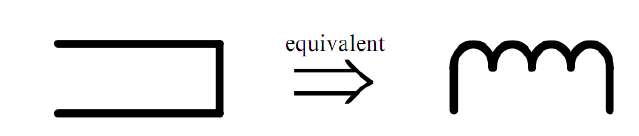
\includegraphics[width=3in]{./images/efield_image1.png}
		\caption{equivalent model of meander line sections}
		\label{fig:efield_fig1}
	\end{center}
\end{figure}


Since the self-resonant frequency of the simple straight line monopole antenna can be modeled as the inductor circuit model, we can use the formula \eqref{eq1} to calculate the self-inductance when the total physical length of the antenna is about $\lambda/4$. 

\begin{equation}\label{eq1}Ls = \frac{\mu}{\pi}0.2384 \lambda (ln(4 \frac{0.2384 \lambda}{d} - 1)) \end{equation}

Where d is the diameter of the radiator of the antenna and $\lambda$ is the required resonant wavelength, the resonant frequency of the antenna can be estimated using an inductor circuit model representation as introduced in figure \ref{fig:efield_fig1}. To determine the inductance in each meandered section, we will use an equivalent transmission line model which has a characteristic impedance given as 

\begin{equation}Z_0 = 276log(\frac{2s}{d})\end{equation}

 where s is the spacing between each meandered section, as a result, the equivalent inductance of each section, Lm, is given as following:

\begin{equation}\label{eq2}Lm = \frac{|Z_0 tanh(\gamma l)|}{\omega} \end{equation}

Where  is the propagation factor of free space, l is the length of each meandered section and is angular velocity, the resonant frequency of the meandered line antenna should have same physical length as the simple straight line monopole antenna, but we need to replace the equivalent inductor Ls by the sum of Ls+NLm, where N is the number of meander sections.

In order to exam the resonant behavior of the meandered line antenna, we will simulate and use optimism method in HFSS to compare each group of meandered antenna parameters given above. M0 to M5 configurations shown in figure \ref{fig:efield_fig2} (Best, Morrow) is applied to observe the variation the resonant frequency of the antenna.[1],[2]

\begin{figure}[h]
	\begin{center}
		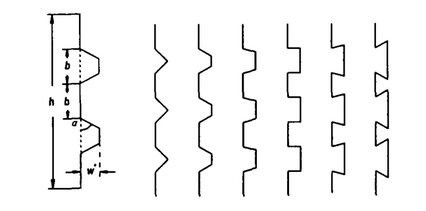
\includegraphics[width=3.4in]{./images/efield_image2.png}
		\caption{meandered monopole antenna geometry}
		\label{fig:efield_fig2}
	\end{center}
\end{figure}

The M0 configuration has a self-resonant frequency at 80MHZ, while the M5 configuration has a self-resonant frequency at 110MHZ. For antenna represented in Fig 1, s is equal to 1cm, L is equal to 4cm, using equation (2) and (3), and the value of Lm is calculated as about 300nH, a comparison table of resonant behavior of different numbers of section is listed in figure \ref{fig:efield_fig3}.

\begin{figure}[h]
	\begin{center}
		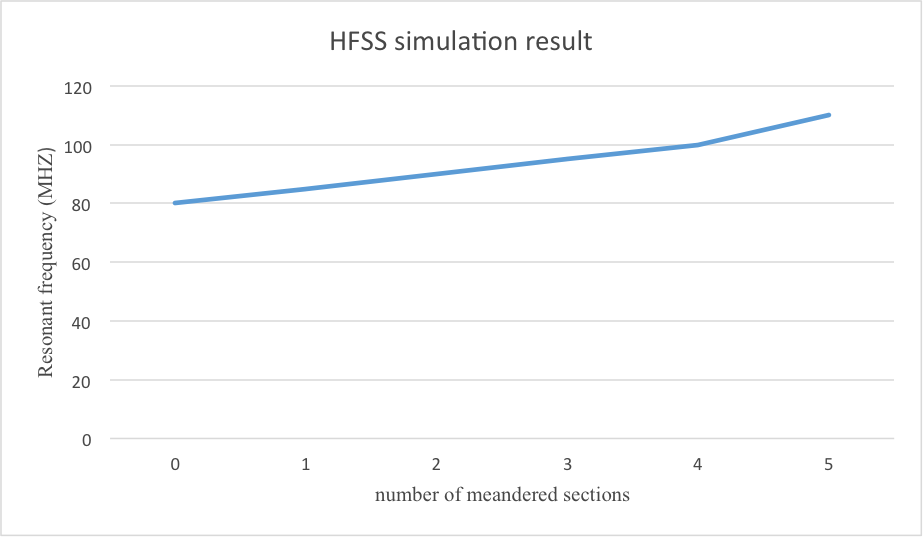
\includegraphics[width=4.3in]{./images/SG_fig3.png}
		\caption{Resonant frequency of meandered line antenna M0 to M5}
		\label{fig:efield_fig3}
	\end{center}
\end{figure}

From figure \ref{fig:efield_fig3}, it is evident that the inductor circuit model representing the meandered antenna provides an acceptable prediction showing a liner increase in resonant frequency as a function of increasing bending sections, however, in the real case, the resonant frequency of the meander line antenna will not linearly increase with the number of sections.[1],[2]

The limitation of inductor circuit model of the meandered antenna is still in examining, we simulated that some of the physical properties varied and the corresponding change of the resonant frequency. Firstly, we change the s in M1 configuration from 1cm to 2cm, the resonant frequency behavior of the antenna versus the meandered sections is shown in figure \ref{fig:efield_fig4}. We can observe that the actual resonant frequency will not precisely change as we seen in figure \ref{fig:efield_fig3}. 

\begin{figure}[h]
	\begin{center}
		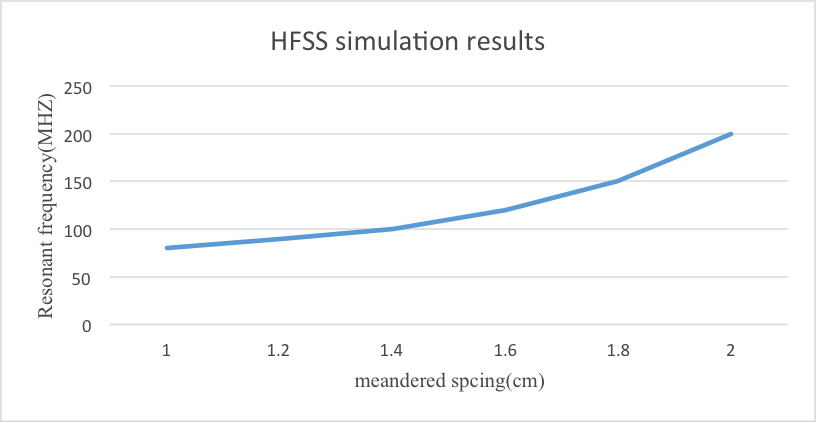
\includegraphics[width=4.3in]{./images/SG_fig4.png}
		\caption{resonant frequency vs meandered spacing}
		\label{fig:efield_fig4}
	\end{center}
\end{figure}

Next, we examined the effect of bending angle changing for each meandered section shown in figure \ref{fig:efield_fig5} [1]

\begin{figure}[h]
	\begin{center}
		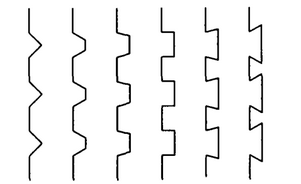
\includegraphics[width=3in]{./images/efield_image4.png}
		\caption{Bending angle when α= 45,60,75,90,120 degree conditions}
		\label{fig:efield_fig5}
	\end{center}
\end{figure}

We bend the antenna for the configuration M5 too see the simulation results in HFSS while keep the total physical length and spacing as the same as the previous model. The relation between bending angle and self-resonant frequency is shown in figure \ref{fig:efield_fig6}.

\begin{figure}[h]
	\begin{center}
		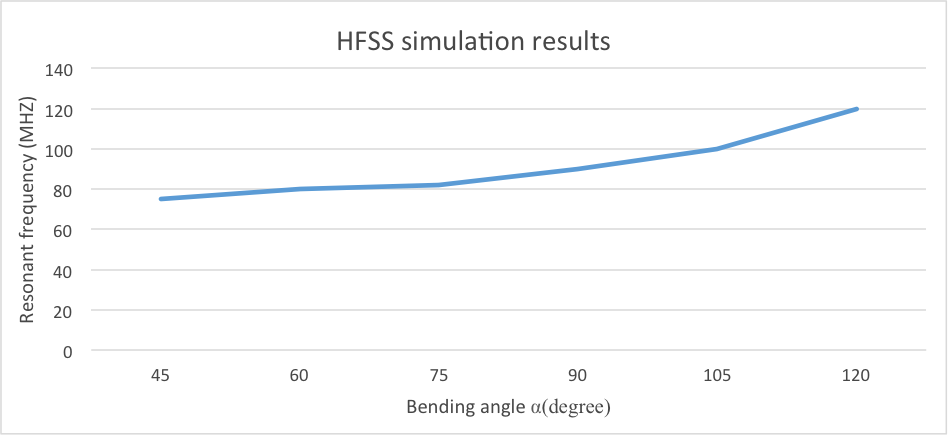
\includegraphics[width=4.3in]{./images/SG_fig5.png}
		\caption{the relation between bending angle and resonant frequency}
		\label{fig:efield_fig6}
	\end{center}
\end{figure}

It is observed that resonant frequency would experience a little fluctuate when the bending angle is changing from 45 to 120 degrees. Nevertheless, we need to obtain a relatively large difference between cross-plane and co-plane polarization, as we can see in Fig.6, the 90 degree bending angle will provide a cancellation of radiation in horizontal axis due to the opposite flowing direction of two current. At the same time, the radiation current will always along a same direction in vertical axis, as a result, the radiation of the 90 degree bending antenna is equivalent to a single line monopole antenna. Furthermore, the 90 degrees bending method will save room on PCB board so that the total physical length of the antenna will get dropped.

\begin{figure}[h]
	\begin{center}
		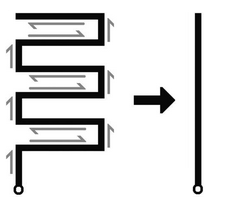
\includegraphics[width=2in]{./images/efield_image5.png}
		\caption{the relation between bending angle and resonant frequency}
		\label{fig:efield_fig7}
	\end{center}
\end{figure}

\subsection{Antenna Building and Testing}

After investigating the effects of numbers of section, section spacing and bending angle, we start to build a meandered antenna on the substrate to satisfy the specification of the antenna parameters. As seen in figure \ref{fig:efield_fig8}, the spacing between each meandered section is 0.5cm, the number of meandered sections is 14 in total, and the s11 graph is shown in figure \ref{fig:efield_fig9} which provide us a return loss below -10dB.

\begin{figure}[h]
	\begin{center}
		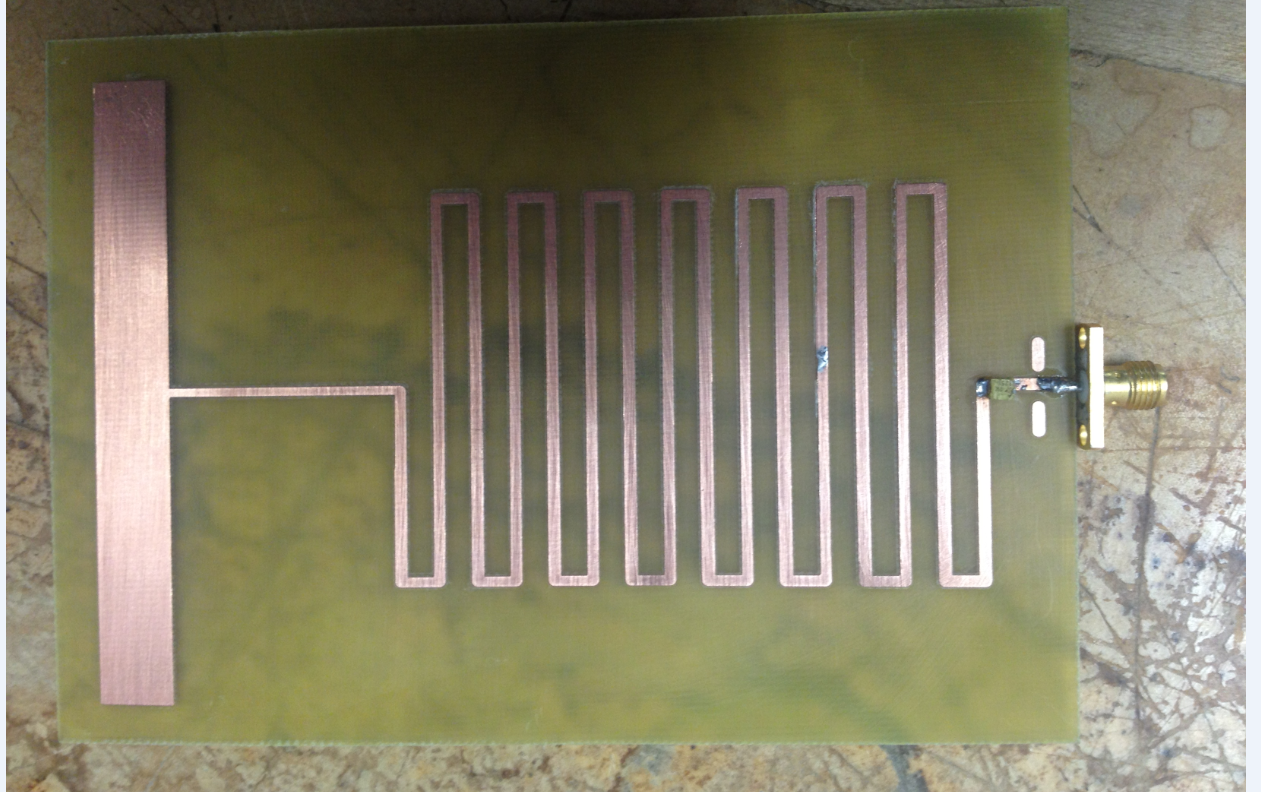
\includegraphics[width=4in]{./images/efield_image6.png}
		\caption{final antenna view}
		\label{fig:efield_fig8}
	\end{center}
\end{figure}

The physical length of this antenna is 80cm in total with the height of 10cm on the substrate, a top loading cap is added at the far end of the antenna to increase the s11 performance. To match up the resonant circuit, we add a 400nH inductor at the feeding point of the antenna. When testing the S12 parameter, we used a $\lambda/4$ dipole antenna as port 2 in HFSS so that the designed antenna is acting as a receiving antenna in the air box. The simulation model is shown in figure \ref{fig:efield_fig9}. And the simulation results are listed in figures \ref{fig:efield_fig10}, \ref{fig:efield_fig11} and \ref{fig:efield_fig12}.

\begin{figure}[h]
	\begin{center}
		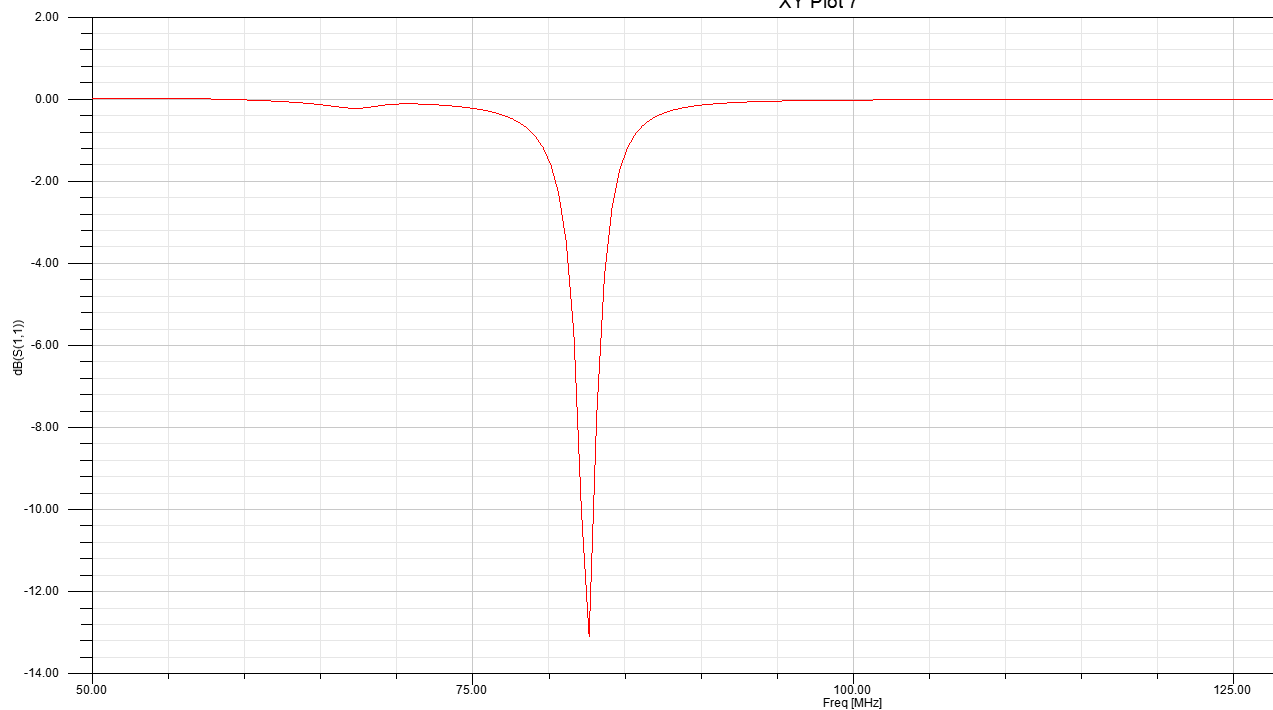
\includegraphics[width=4.3in]{./images/efield_image7.png}
		\caption{S11 curve for meandered antenna in HFSS}
		\label{fig:efield_fig9}
	\end{center}
\end{figure}

\begin{figure}[h]
	\begin{center}
		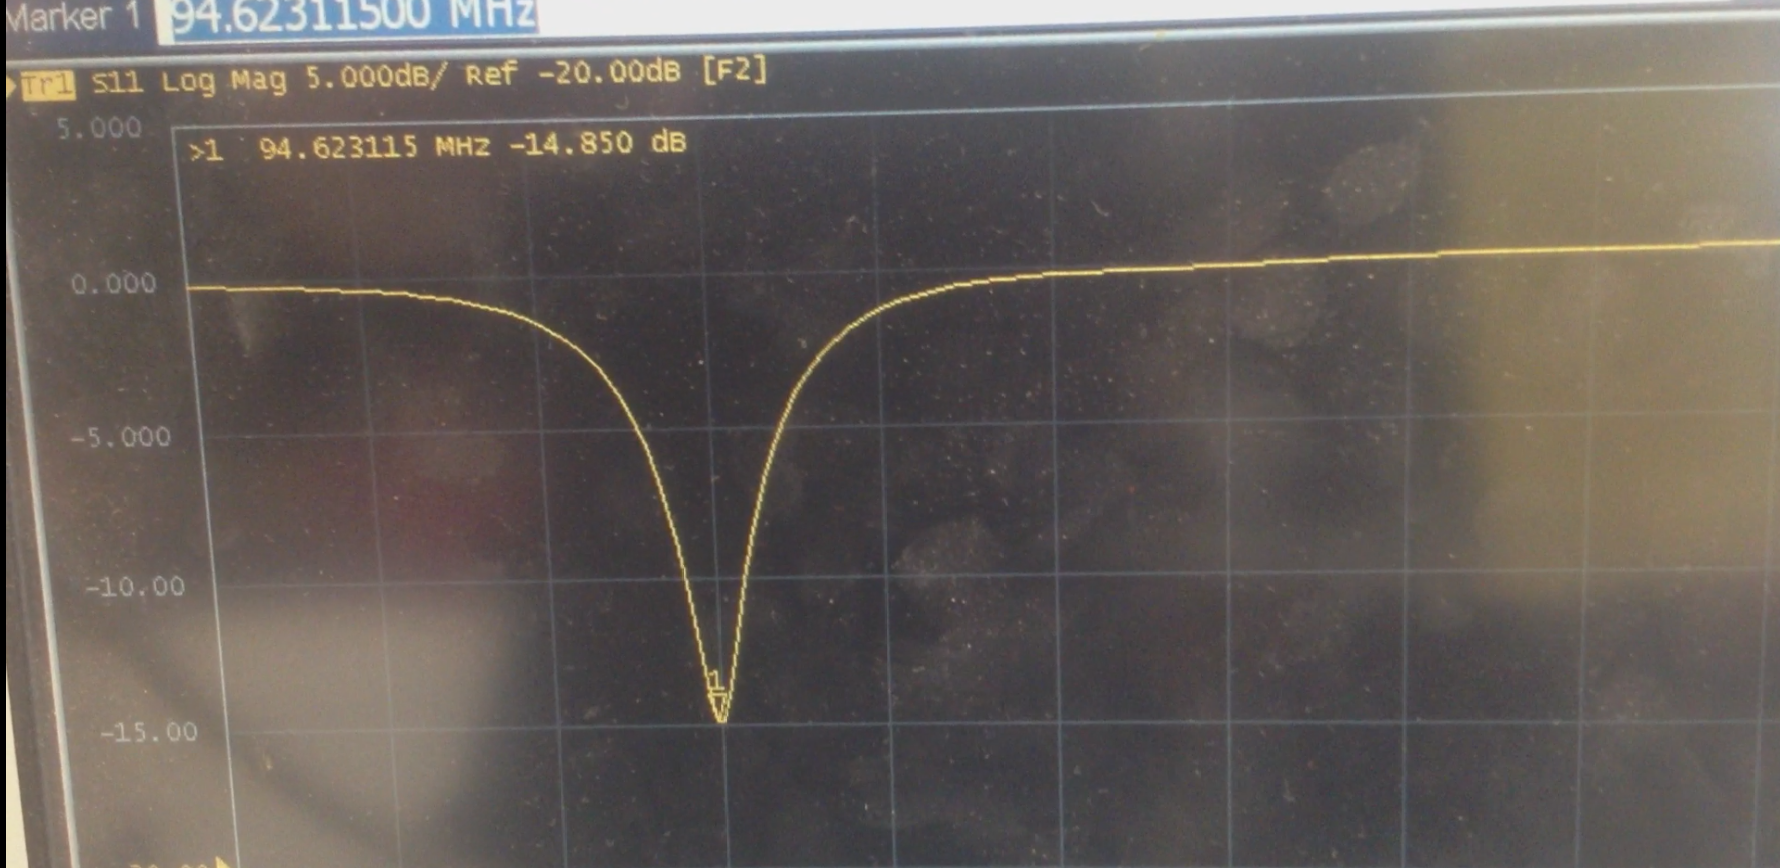
\includegraphics[width=4.3in]{./images/efield_image8.png}
		\caption{ S11 curve for real testing results}
		\label{fig:efield_fig10}
	\end{center}
\end{figure}

In the real testing, the resonant frequency got shifted to 95MHZ due to the inaccurate selection of the inductor value, since we can only get 330nH or 470nH one from the lab, the result frequency will not located in 80MHZ.

\begin{figure}[h]
	\begin{center}
		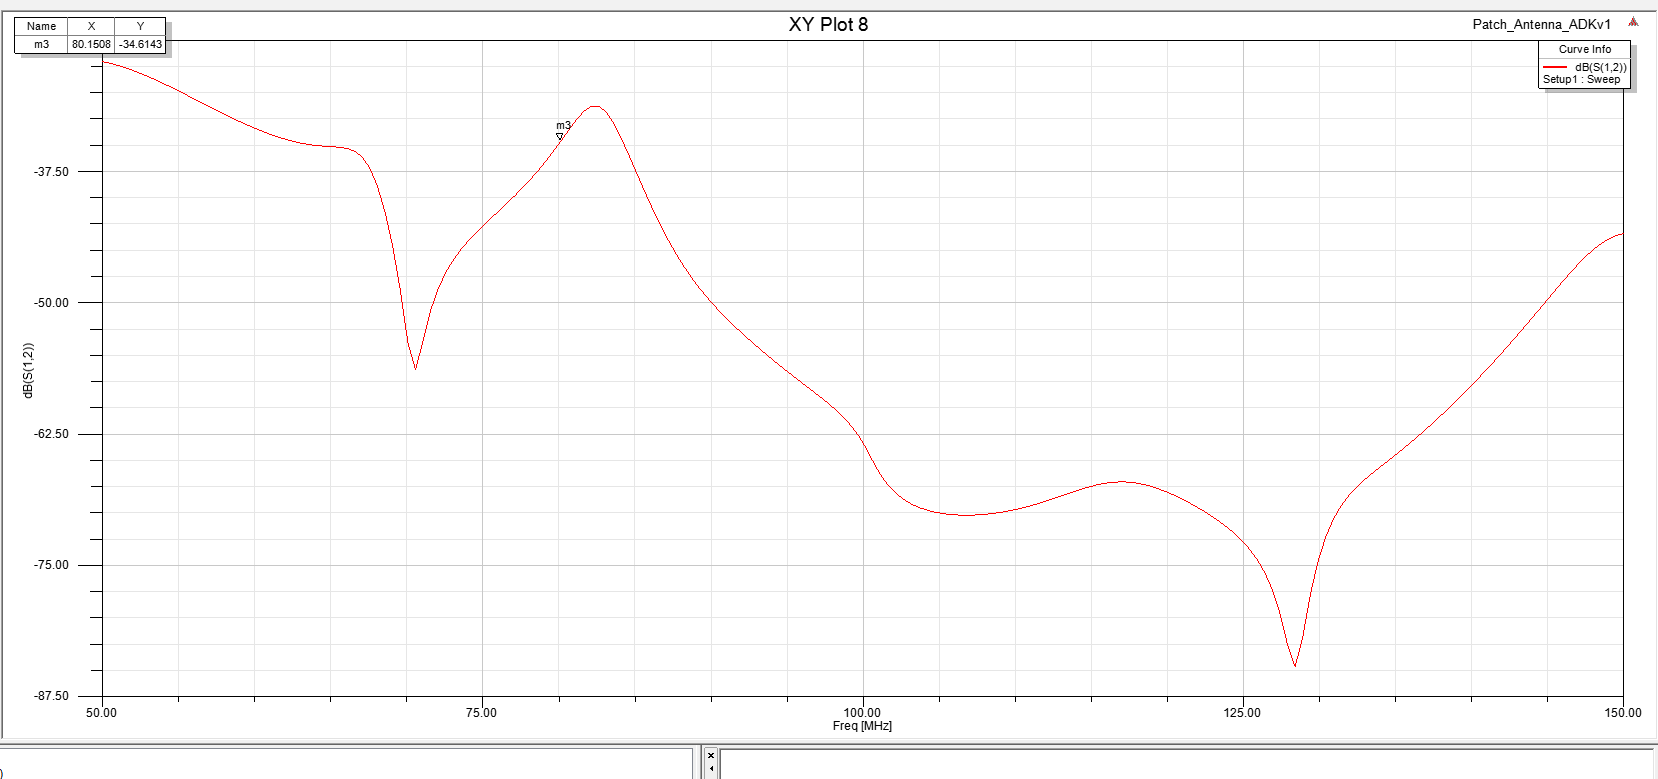
\includegraphics[width=4.7in]{./images/efield_image9.png}
		\caption{ S12 curve for cross-plane polarization in HFSS}
		\label{fig:efield_fig11}
	\end{center}
\end{figure}

\begin{figure}[h]
	\begin{center}
		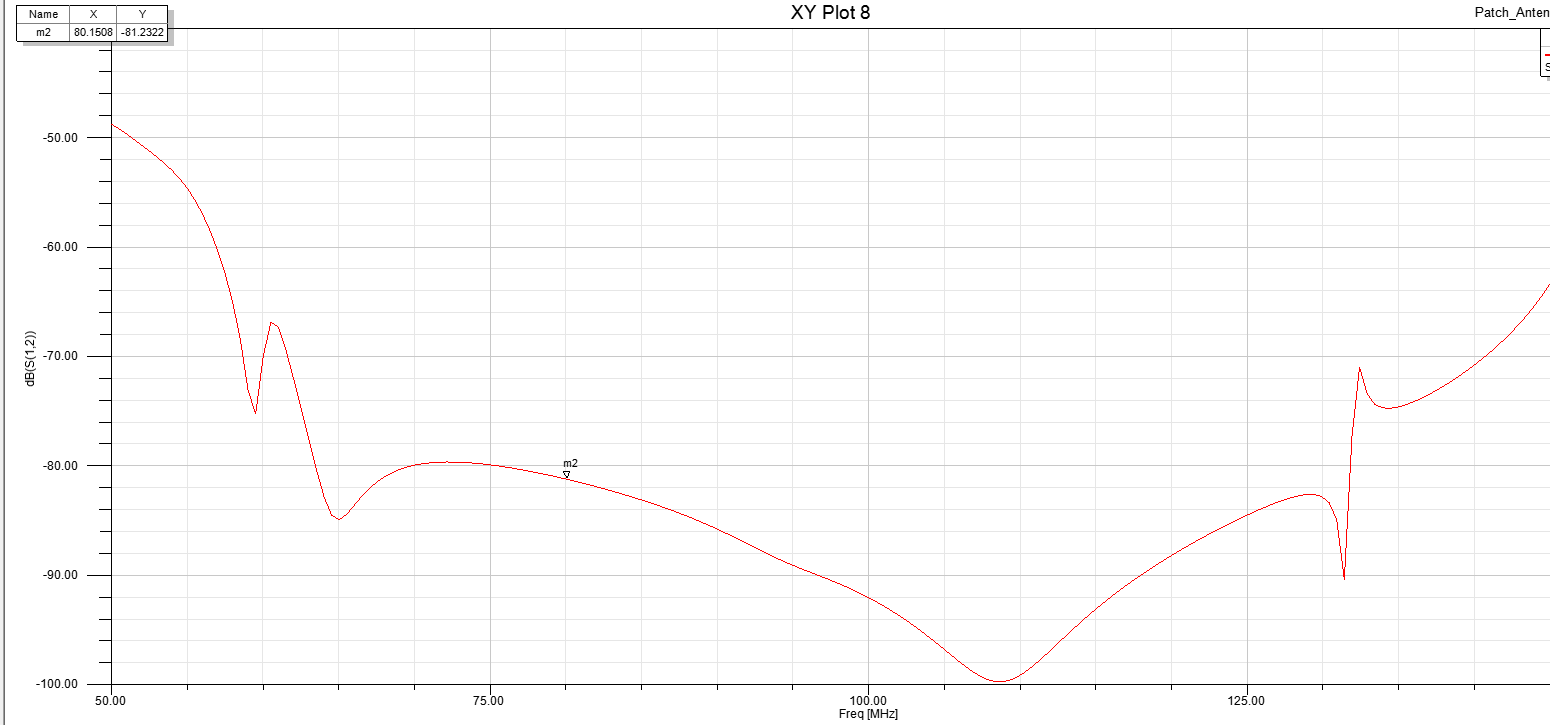
\includegraphics[width=4.7in]{./images/efield_image10.png}
		\caption{S12 curve for co-plane polarization in HFSS}
		\label{fig:efield_fig12}
	\end{center}
\end{figure}

\clearpage

\begin{figure}[h]
	\begin{center}
		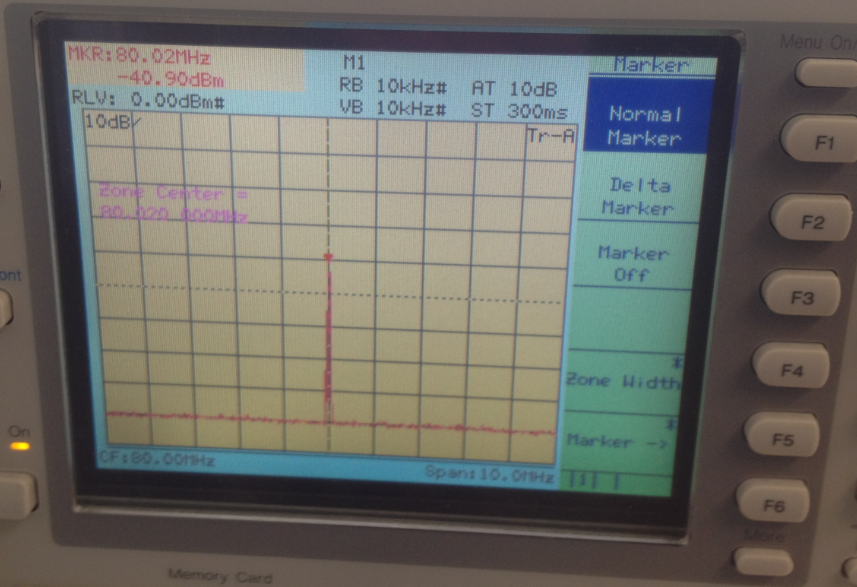
\includegraphics[width=3.4in]{./images/efield_image11.png}
		\caption{S12 curve for cross-plane polarization in real test}
		\label{fig:efield_fig13}
	\end{center}
\end{figure}

\begin{figure}[h]
	\begin{center}
		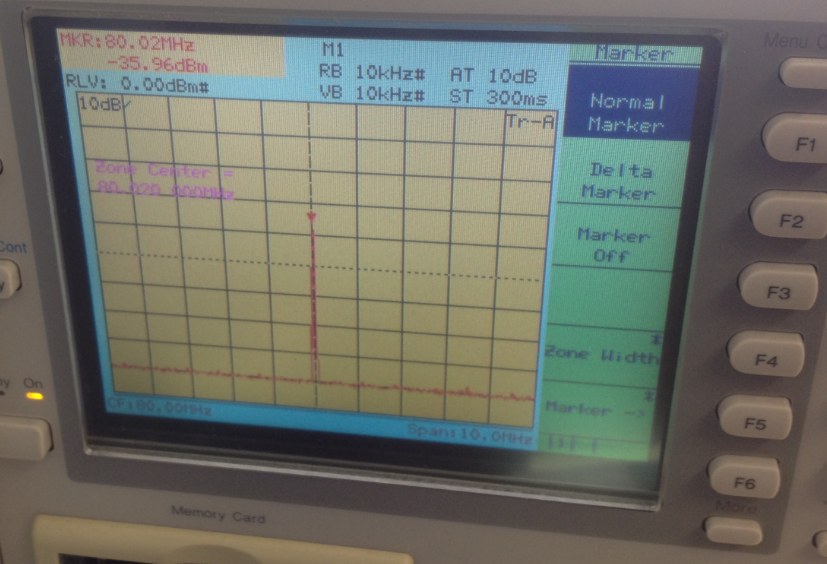
\includegraphics[width=3.4in]{./images/efield_image12.png}
		\caption{S12 curve for co-plane polarization in real test}
		\label{fig:efield_fig14}
	\end{center}
\end{figure}

\clearpage

As a conclusion, for s12 curves, in HFSS the results is pretty good that difference between co-plane and cross-plane of s12 is about 15dB, but in the real test, the difference is 5db, the cause for the difference in quantity is from the non-ideal air box and ground plane from the lab comparing to the ideal ones in HFSS. Further improvement for the testing method is still required.



